\documentclass[a4paper]{report}



    \usepackage[colorinlistoftodos]{todonotes}
 
	\usepackage[utf8]{inputenc}
	\usepackage[T1]{fontenc}
    \usepackage[frenchb]{babel}
    \usepackage{textcomp} 
	\usepackage[top=3cm,left=3cm,right=3cm,bottom=2cm]{geometry}
    \usepackage{lmodern}
    \usepackage{sectsty}
    \usepackage{nicefrac}
	\usepackage{graphicx}
    \usepackage{lastpage}
    \usepackage{fancyhdr}
    \usepackage{amsmath}
    \usepackage{amssymb}
    \usepackage{amsfonts}
    \usepackage{capt-of}
    \usepackage{caption}
    \usepackage{tikz}
    \usepackage{multirow}
	\usepackage{todonotes}    
    
    \usepackage{fancyvrb} % pour forcer les verbatim sur une seule page
    \usepackage{url}
    
    \usepackage{subfigure}
    %\usepackage{subcaption}
    
    \newcommand\matlab{MATLab\textsuperscript{\textregistered}}




\title{Premier jet du Rapport de projet de M1: Réseau periodiques et modes localisés }
%\subtitle{Basis of room acoustics: TP1}

\author{Thomas Lechat \& Alice Dinsenmeyer}

\begin{document}
\maketitle
\tableofcontents

\chapter*{Remerciements}

\chapter*{Abstract en anglais}
même chose que l'intro + résultats principaux \\


\chapter*{Introduction}


La propagation dans les réseaux n'est pas un sujet nouveau: celui-ci a déjà été abordé en profondeur notamment dans des recherches en cristallographie et en électromagnétisme. Cependant sont pendant acoustique à fait l'objet de peut de recherches.

L'étude de la propagation acoustique dans les réseaux est un domaine complexe des lors que les éléments constitutif du réseau disposent de leurs propres fréquences de résonance. En effet, 2 types de bandes interdites sont alors présentes et peuvent interagir: les bandes de Bragg lié à la géométrie du réseau et les bandes interdites liés au comportement fréquentiel des éléments du réseau. Si on défaut est ajouté dans le réseau, il peut alors ce produire un phénomène de localisation de la pression dans le tube: c'est ce qu'on appelle un mode localisé (ou mode de défaut).

Ce travail s'inscrit dans le cadre de recherche sur les méta-matériaux composés de structures résonantes localisés. Ce genre de matériaux dispose de propriétés uniques tels que la réfraction négative ou encore des matériaux super-absorbant. Notre projet consiste à mieux comprendre le phénomène de mode localisé afin que des chercheurs puissent exploiter les résultats obtenues en y ajoutant des phénomènes d'acoustique non-linéaire.

\bigskip
Le but du projet est donc d'étudier la propagation dans un réseau composés de résonateurs de Helmholtz en prenant en compte les pertes visco-thermique intrinsèque à la propagation dans ce type de structure. Une fois la théorie sur les réseaux périodiques assimilé, une étude sur l'ajout d'un défaut dans le réseau sera effectuée. Des simulations seront confrontés à des mesures sur un réseau se trouvant au laboratoire d'acoustique de l'université du Maine.

%\begin{itemize}
%
%\item domaine de recherche: méta-matériaux, filtrage analogique, tout les phénomènes de propagation.
%\item Citation des sources => optique puis electromagnetique puis acoustique
%\item but: comprendre propagation dans réseau et visualisation expérimental de mode localisé
%\item plan: Approche théorique de la propa dans réseau ac, ajout de singularité pour mode localisé, expérimentation
%\end{itemize}
\chapter{Théorie d'un réseau acoustique de résonateur de Helmholtz fini}
Le but du projet est de caractériser un réseau de résonateur de Helmholtz placés sur un guide d'onde. On dispose pour cela d'un banc de mesure représenté figure ~\ref{schema_infini}. Une simulation de la propagation dans le réseau pourra donc être confronté à une expérience.

\begin{figure}[!ht] \centering
\includegraphics[scale=0.5]{./images_chp1/schema_reseau_infini.png}
\caption{\label{schema_infini} Schéma du réseau de résonateurs de Helmholtz.}
\end{figure}


\section{Mise sous forme matricielle}
On s’intéresse ici a la mise sous forme matricielle du problème de la propagation acoustique dans le réseau periodique vu ci-dessus. Le but étant de mettre le système sous la forme suivante:
\begin{equation}
\begin{pmatrix} P_{out} \\ U_{out} \end{pmatrix} =\begin{pmatrix} a & b \\ c & d \end{pmatrix}^N \begin{pmatrix} P_{in} \\ U_{in} \end{pmatrix} = \begin{pmatrix} A & B \\ C & D \end{pmatrix} \begin{pmatrix} P_{in} \\ U_{in} \end{pmatrix} 
\end{equation}

Cette matrice dispose en effet de propriétés intéressantes et l'étude du système sera grandement facilité par ce formalise.

Pour cela, les 2 éléments du réseau (guide et résonateur) doivent être mis sous forme matricielle puis multipliés.

\subsection{Le guide d'onde}
La solution de la propagation dans un guide d'onde peux être facilement déduite de l'équation d'onde suivante:
\begin{equation}
\frac{\partial ^2 p}{\partial x^2} -\frac{1}{c^{2}} \frac{\partial ^2 p}{\partial t^2}= 0
\end{equation}

On se place en régime harmonique et on note $\Gamma = jk$ la constante de propagation du système. D’où les solutions (vitesses calculées avec l'équation d'Euler:

\begin{eqnarray*}
\begin{cases}
p(x_1)  =  C1 e^{-\Gamma x_1} + C2 e^{\Gamma x_1} \\
v(x_1)  =  -\frac{1}{j\omega\rho} [ -\Gamma C1 e^{-\Gamma x_1} + \Gamma e^{\Gamma x_1}]\\
p(x_2)  =  C1 e^{-\Gamma x_2} + C2 e^{\Gamma x_2} \\
v(x_2)  =  -\frac{1}{j\omega\rho} [ -\Gamma C1 e^{-\Gamma x_2} + \Gamma e^{\Gamma x_2}]
\end{cases}
\end{eqnarray*}
 
On pose $x_1 - x_2 = L$. Tous calculs faits, on trouve finalement:
\begin{eqnarray*}
\begin{pmatrix} p(x_1) \\ v(x_1) \end{pmatrix} = \begin{pmatrix} \cosh(kL) & \frac{j\omega\rho}{k} \sinh(k L) \\  \frac{k}{j\omega\rho}\sinh(k L) & \cosh(k L) \end{pmatrix} \begin{pmatrix} p(x_2) \\ v(x_2) \end{pmatrix}
\end{eqnarray*}

La première fréquence de coupure du guide est donc d'environ $4kHz$ pour les dimensions du réseau que nous considérons. Dans la suite, on supposera donc que seul le mode plan est propagatif. Les simulations et mesures ne seront donc faite que sur une bande de fréquences allant de $0$ à $1~kHz$.

\subsubsection{Ajout des pertes}

Pour prendre en compte les pertes, on modifie l'expression de la constante de propagation et de l'impédance caractéristique. Les expressions utilisées se trouvent en [A1]. on a donc:
\begin{eqnarray*}
 k =  \frac{\omega}{c_0} \left( 1 + \frac{\beta}{s}(1+(\gamma-1)/ \chi \right) \\
 Z_c =  \frac{\rho c_0}{S} \left( 1 + \frac{\beta}{s}(1-(\gamma-1)/ \chi \right) 
\end{eqnarray*}

Et où on a:
\begin{itemize}
 \item  $s=R/ \delta$ avec $\delta = \sqrt{\frac{2 \mu}{\rho \omega}}$
 \item  $\chi = \sqrt{P_r}$ ou $P_r$ est le nombre de Prandtl
 \item $\beta = (1-j)/\sqrt{2}$ 
 \item $\mu$ la viscosité de l'air
\end{itemize}

Du fait de la géométrie assez complexe du système, ces pertes ne peuvent pas être négligées comme cela peux être souvent le cas en acoustique.

\subsection{Le résonateur}
Le résonateur de Helmholtz est considéré dans le réseau comme un changement ponctuel d'impédance. Cette impédance peux etre calculée via la formule de l'impédance ramenée ~\ref{imp_ramenee}. De plus, les dimensions utilisées dans la suite sont corrigées afin de prendre en compte les corrections de longueurs liés à la géométrie du problèmes. Ces formules de corrections sont disponibles en annexe 2.
\begin{eqnarray}
Z{x_1}=\frac{jZ_c tan(kL)+Z_{x_2}}{1+j\frac{Z_{x_2}}{Z_c}tan(kL)}.
%\label{imp_ramenee}
\end{eqnarray}

Si on suppose que le résonateur est constitué d'une parois rigide et de 2 tubes, on peux calculer sont impédance comme suit:

\begin{eqnarray*}
\begin{pmatrix} P_2 \\U_2 \end{pmatrix} & = & \begin{pmatrix} \cos(k l) & j Z_{c_1} \sin(k l) \\ \frac{1}{Z_{c_1}} \sin(k l) & \cos(k l) \end{pmatrix} \begin{pmatrix} \cos(k L) & j Z_{c_2} \sin(k L) \\ \frac{1}{Z_{c_2}} \sin(k L) & \cos(k L) \end{pmatrix} \begin{pmatrix} P_1 \\ 0  \end{pmatrix} \\
\begin{pmatrix} P_2 \\U_2 \end{pmatrix} & = & \begin{pmatrix} r_1 & r_2 \\ r_3 & r_4 \end{pmatrix} \begin{pmatrix} P_1 \\ 0  \end{pmatrix} \\
~ & \Leftrightarrow & Z_{resonateur} = \frac{A}{C}
\end{eqnarray*}

Si on ajoute un résonateur en parallèle au guide, on a toujours continuité des pressions mais plus des vitesses. On a donc la matrice de transfert pression-vitesse suivante pour un résonateur dans le réseau:

\begin{eqnarray*}
M_{resonateur} = \begin{pmatrix} 1 &  0 \\ 1 /Z_{resonateur} & 1  \end{pmatrix}\\
\end{eqnarray*}

\section{Étude du réseau fini}

Une fois les matrices de guide et de résonateur connues, il suffit alors de les multiplier afin d'obtenir la matrice d'une cellule du réseau. C'est sur l'étude de cette matrice que ce base les analyses de cette section. En effet, l'étude d'une seul cellule permet d'analyser le cas d'un réseau infini de cellules.

Dans la suite les paramètres de la simulation sont ceux du de l'expérience dont nous disposons. Ces paramètres sont disponible en annexe 2.

\subsection{Équation de dispersion}
On peux déduire de la matrice de transfert l'équation de dispersion pour le réseau à N cellules, on a en effet:
\begin{equation}
\cos(NkL) = \frac{A+D}{2} 
\end{equation}

Ainsi, on peux remonter à une expression de $kL$ en fonction de la fréquence. En particulier, les zones ou $kL$ devient imaginaire nous intéresse particulièrement car cela induit une décroissance exponentielle de l'onde de propageant dans le guilde. Ces bandes sont visible sur la figure ~\ref{bande_bragg} et sont appelées les bandes de Bragg.

\todo{une figure de l’équation de dispersion avec bande de bragg}

\subsection{Bande de Bragg}
Ces bandes de Bragg apparaissant dès qu'un élément est présent dans un réseau et ce de manière periodique. L'énergie de l'onde reste "enfermée" entre chaque éléments du fait que la longueur d'onde correspond à la moitier de l'espacement entre 2 éléments.  \todo{vérifier ça}.
 

\subsection{Bande interdites liés aux résonateurs}
L'équation de dispersion est cependant plus difficile analyser qu'il n'y parait du faite que ce sont des résonateurs qui servent d’éléments au réseau. Hors ce ci ont une impédance négligeable dès lors que la fréquence d'analyse ce trouve suffisamment éloignées des fréquences de résonances. 

De plus le résonateur étant par nature un système résonant, il peux lui aussi induire une absorption de l'énergie de l'onde sur certaines fréquences.

Il y a donc 2 phénomènes qui peuvent induire des bandes interdites, d'une part les bandes de Bragg liés a la géométrie du réseau et d'autre part l'énergie absorbée par les résonateurs.
\todo{Double figure explicative avec les 2 types de bande}.


\subsection{Réflexion et transmission du réseau}
On peux enfin tracer le coefficient de réflexion et de transmission du réseau complet. En effet, on a:
\begin{eqnarray}
T & = & \frac{2}{A + B/Z_c + C Z_c + D} \\
R & = & \frac{A + B / Zc_ - C Z_c -D}{A + B/Z_c + C Z_c + D} 
\end{eqnarray}

On obtient des résultats de ce type:
\todo{figure de Réflexion et transmission type}

\chapter{Ajout d'une singularité dans le réseau}
La seconde partie de ce projet est une étude portant sur l'observation d'un mode localisé dans le réseau précédemment étudié. Pour cela, un résonateur est modifié de façon à créer une singularité dans le réseau. \\
Le banc de manipulation ne nous permet de modifier que la longueur des cavités des résonateurs et non leur position. C'est donc en changeant ce paramètre que sera introduite et étudiée la singularité. La longueur de la cavité singulière est notée $L_{c_{s}}$.\\

En fonction du choix de la longueur de la cavité singulière -et donc de la fréquence de résonance du résonateur associé- différents phénomènes peuvent être observés. 


\section{Cas d'une singularité hors bande de Bragg}


\section{Cas d'une singularité dans la bande de Bragg}

\section{Calcul numérique de la pression dans le réseau}

\section{Étude de l'influence de la position du défaut}
\chapter{Visualisation expérimental d'un mode localisé}
Différents problèmes rendent la mesure d'un mode localisé difficile.

Tout d'abord il n'est pas trivial de trouver une configuration qui permette la génération d'un mode localisé car c'est un phénomène difficile à visualiser et ce même en simulation. La fréquence de résonance du défaut doit se trouver sur le bords d'une bande interdite (à l'intérieur) afin de pouvoir la visualiser sur les coefficients de transmission et réflexion. En effet, la propagation de l'onde dans le réseau est difficile: la bande interdite rend la décroissance de l'onde exponentielle. Par conséquence, exciter le mode de défaut est difficile et même s'il est excité la pression reste localisé. Celle-ci n'est alors pas visible sur les coefficients de transmission et de réflexions qui sont issues de mesures à l'entrée et la sortie du réseau sauf dans le cas d'un réseau constitué de peu d’éléments et avec un défaut en bord de bande.


\subsection{Protocole expérimental}
Le banc de mesure utilisé est constitué d'un tuyau de 60 trous sur lequel peuvent être fixé des résonateurs variablesb (les dimensions sont présents en annexe) ou bien des bouchons. La source utilisée est celle du capteur d'impédance: celui-ci est fixé à une des extrémités du réseau et est relié à une carte d'acquisition piloté par le logiciel spécialisé du CTTM. Ce capteur dispose de 2 microphones et permet donc de calculer directement le coefficient de réflexion du réseau. Afin de pouvoir calculer le coefficient de transmission, un autre microphone est ajouté $10~cm$ après le dernier résonateur.
\todo{citer une annexe sur la démo du coefficient de transmission et mettre la bonne annexe sur les dims des resonateurs}

\bigskip

A l'autre extrémité du réseau se trouve une embouchure de sortie anéchoïque préalablement réglée afin que le coefficient de réflexion au bout du réseau soit le plus faible possible.
\todo{une annexe sur la source anéchoi => explication sur le reglage+figure?}


\section{Mesure du coefficient de réflexion et de transmission du réseau}
On s'intéresse tout d'abord à la mesure du coefficient de réflexion et de transmission dans le réseau. Bien qu'un mode localisé soit dure à observer dans ces conditions, le but est de chercher la fréquence précise à la quelle celui-ci à lieu afin de pouvoir par la suite mesure ce mode à l'intérieur du réseau. Pour cela on ne prend que 5 résonateurs (avec un défaut sur le troisième) afin que le mode localisé puisse "déborder" sur les bords du réseau et ainsi qu'il soit mesurable (dans cette configuration l'atténuation lié au bandes interdites est moins importante). Les résonateurs ont une longueurs de cavité de $16~cm$ et le défaut de $8~cm$. Les courbes figure ~\ref{ref1} et ~\ref{trans1} correspondent aux coefficients de réflexion et de transmission pour cette configuration.

\begin{figure}[!h]
\centering
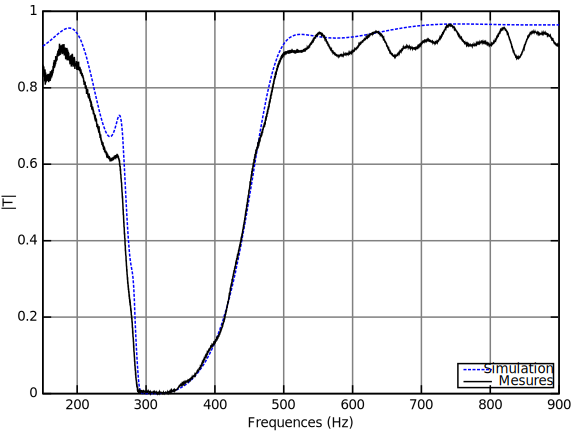
\includegraphics[scale=0.4]{images_chp3/5HR165_nodefect.png}\hfill
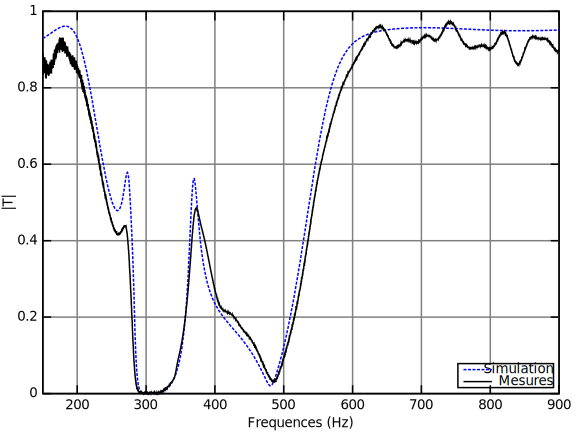
\includegraphics[scale=0.4]{images_chp3/5HR165_8cm_pos3.png}
\caption{\label{ref_trans1} Coefficient de transmission du réseau dans un cas sans défaut et avec défaut. Les courbes de simulations et de l’expérience sont superposées.}
\end{figure}

On constate qu'un pic de transmission est visible dans la bande interdite tant théoriquement qu'expérimentalement: le défaut permet à l'onde de traverser le réseau pour une fréquence donnée alors que dans le cas ou celui-ci n'est pas présent aucune transmission n'est possible. Ce comportement laisse supposer qu'un mode localisé est présent au niveau du défaut: si on augmente le nombre de résonateur, l'atténuation est plus forte et le pic disparaît, le mode est alors complètement localisé.

Ces résultats se retrouvent aussi sur la réflexion.
%
%\begin{figure}
%\centering
%\includegraphics[scale=0.3]{•}\hfill
%\includegraphics[scale=0.3]{•}
%\caption{\label{ref_trans1} Coefficient de transmission du réseau dans un cas sans défaut et avec défaut. Les courbes de simulations et de l'expériences sont superposées.}
%\end{figure}
\todo{coefficient de réflexion  pour ce truc la}

\section{Mesure d'un mode localisé par insertion de capteur dans le réseau}
Une fois la fréquence du mode de défaut relevée sur les coefficients de réflexions et transmissions on augmente le nombre de résonateurs de part et d'autre du défaut afin de créer un mode complètement localisé. Afin de pouvoir quand même exciter le mode localisé, une source est placé dans un des orifices au voisinage du défaut. Un microphone est inséré dans le réseau afin de mesure la pression en n'importe quel point. La pression RMS mesurée dans le tube est représenté figure ~\ref{p_tube} pour une configuration avec et sans défaut.

\begin{figure}[!h]
\centering
\includegraphics[scale=0.5]{./images_chp3/non_norm_lin.png}
\caption{\label{_tube} Pression RMS mesurée dans le réseau afin de mettre en évidence un mode localisé.}
\end{figure}

On constate que les niveaux de pression mesurés sont près de 10 fois plus élevé dans le cas ou un défaut est présent. De plus, la décroissance à mesure qu'on s'éloigne du défaut est très importante: on est donc bien en présence d'un mode localisé. Il est a noté que dans cette configuration le niveau maximum dans le réseau ne ce situe pas au niveau de la source mais du défaut (ce qui n'est pas le cas quand il n'y a pas de défaut).

\addcontentsline{toc}{section}{\textbf{Conclusion}}
\chapter*{Conclusion}

Ce projet a permis l'étude d'un réseau périodique de résonateurs de Helmholtz en prenant en compte les pertes visco-thermiques. 

Dans un premier temps, un réseau périodique infini a été étudié afin de se familiariser avec le formalisme matriciel (onde de Bloch): celui-ci est adapté pour décrire ce genre de système. Les simulations faites sur la base de ce modèle théorique ont été en parfait accord avec des mesures effectuées sur le banc d'expérience du LAUM\footnote{\samepage Laboratoire d'Acoustique de l'Université du Maine}. Une étude succincte d'un faible désordre dans le réseau a également été abordée : un désordre sur la position des résonateur affecte les bandes de Bragg, tandis qu'un désordre sur la longueur des cavités modifie les bandes interdites liées à l'impédance des résonateurs.\\

 
Dans un second temps, un défaut a été ajouté dans le réseau afin de générer un mode localisé. Là encore, les simulations sont en accord avec les expériences. Bien que le phénomène soit difficile à observer du fait de la localisation de la pression dans le tube à cause des bandes interdites, les mesures sur un réseau avec un faible nombre de résonateurs ont permis de mettre en évidence l’existence d'un mode de défaut sur les coefficients de transmission et réflexion et de connaître la fréquence exacte d’excitation du mode. Il a alors été possible de mesurer la pression dans le tube en excitant près du défaut à cette fréquence. La différence d'ordre de grandeur des pressions entre un réseau avec et sans défaut s'est montrée flagrante et a corroboré les expériences précédentes, montrant qu'il s'agissait bien d'un mode de défaut.\\

Ces travaux peuvent avoir pour suite l'ajout de phénomènes non-linéaires afin de créer des filtres intéressants à appliquer dans la création de méta-matériaux. Le résonateur de Helmholtz n'étant pas linéaire pour de grandes amplitudes, sa fréquence de résonance s'abaisse quand l'amplitude augmente. Plusieurs applications peuvent donc découler de ce phénomène.

Par exemple, dans le cas d'un résonateur dont la fréquence est dans une bande interdite en amplitude faible, cette résonance pourra ne plus être dans une bande interdite pour une amplitude plus forte : un filtrage en amplitude est alors possible (filtrage dynamique).


De plus, une génération d'harmoniques supérieurs par ce même résonateur est possible en forte amplitude. Ainsi, si une source excite ce défaut, engendrant des harmoniques supérieurs qui ne sont pas dans une bande interdite, la propagation de ces harmoniques est possible. Mais si ce résonateur est placé loin de la source, l'amplitude d'excitation au niveau du défaut sera très faible, et les harmoniques ne seront pas générés. Il est donc possible de créer des systèmes asymétriques sur ce principe.








\chapter*{Annexes}

\section*{Terminaison anéchoïque}
\label{term_anecho}
La terminaison anéchoïque est constituée de fin tissu métallique résistif auquel vient s'ajouter une cavité de section variable qui crée une discontinuité de section. Afin de fixer cette dernière on procède au calcul du coefficient de réflexion du réseau sans aucun résonateur (juste le tube). Le but est de voir quel est l'impact de l'onde réfléchie par la sortie anéchoïque sur l'entrée du réseau. Après réglage, la courbe de réflexion figure~\ref{fig_term_anecho} est finalement obtenue.

\begin{figure}[!h]
\centering
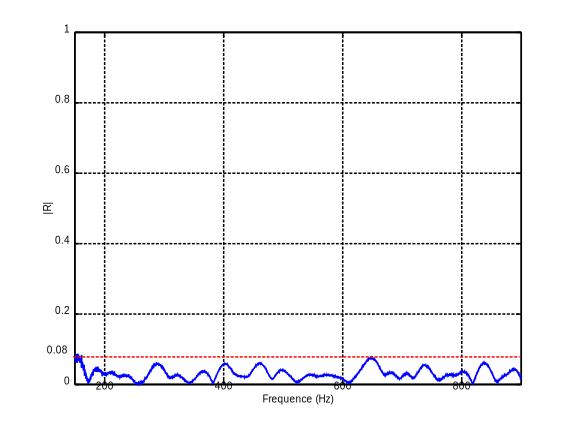
\includegraphics[scale=0.4]{./images_annexe/anecho.png}
\caption{\label{fig_term_anecho} Coefficient de réflexion pour le réseau sans résonateur avec une terminaison anéchoïque adaptée.}
\end{figure}

On constate que le coefficient de réflexion ne dépasse jamais 0.08 ce qui semble tout à fait acceptable afin de considérer la sortie comme anéchoïque dans le reste du projet.

\section*{Paramètres du réseau étudié}
\label{annexe_corr}
La liste des dimensions du réseau utilisé lors des expériences et des simulations est la suivante:
\begin{itemize}
\item Le guide a un rayon de $R_t = 2.5~cm$ et une épaisseur de $ep = 0.5~cm$.
\item Les résonateurs sont composés de 2 tubes: le col de $R_n = 1~cm$ de rayon et $L_n = 2~cm$ de longueur, la cavité de $R_c = 2.15~cm$ de rayon et de longueur variable $L_c$. C'est cette dernière longueur qui permet de faire varier la fréquence de résonance du résonateur. 
\end{itemize}

\bigskip
Les corrections apportées aux cols des résonateurs sont les suivantes:
\begin{eqnarray*}
l_1 & = &  0.82 \left[ 1 - 1.35 \frac{R_n}{R_c} + 0.31 \left(\frac{R_n}{R_c} \right)^3  \right] R_n \\
l_2 & = &  0.82 \left[ 1 - 0.235 \frac{R_n}{R_t} - 1.32 \left( \frac{R_n}{R_t} \right)^2 +1.54 \left( \frac{R_n}{R_t}\right)^3 - 0.86 \left( \frac{R_n}{R_t}\right)^4  \right] R_n \\
L_{corr} & = &  l_1 + l_2
\end{eqnarray*}
Celles-ci sont dues aux discontinuités de section à l'entrée et la sortie du col. Ces discontinuités entraînent une augmentation de la longueur effective de part et d'autre du col.
\textbf{Notations}

résonateurs : 
$L_{n}$ : longueur du col
$R_{n}$ : rayon du col
$L_{c}$ : longueur de la cavité
$R_{c}$ : rayon de la cavité
$S_{n}$ : section du col
$S_{c}$ : section de la cavité
$Z_{c}$ : impédances carac du col. De même pour n

impédance quelconque au point $x_{0}$ : $Z(x_{0})$

impédance du résonateur : $Z_{r}$




\bibliographystyle{plain}
\bibliography{biblio}
\end{document}